
% PAGES: 15
\chapter{Literature Review} % 2 Seiten -> To Introduction? (act sum 2)
\label{mt:c:LiteratureReview}

The realization of a distributed optical error correction scheme for \gls{UAV}
contains several challenges of different topics of technical information
technology, which have to been introduced for this project in the context of a
literature survey. These topics are related to the focus to create a
simulation. That means the theory of function and the complexity of these topics
should be examined, as also the possibilities of simplification.

The first part of the survey will introduce the basic quadrocopter flight
dynamics and approaches to derive the mathematical model of motion. The result of
this model will be the \gls{EOM} in a form which can be used for simulation and
reflects as much as possible the reality.

A comparison between the researched existing visual approaches for error correction of
\gls{UAV}, will be the focus of the second part of this survey. Thereby, the strengths
and weaknesses in focus of different aspects have to be given. Furthermore, this
part will introduce optical movement detection technique which will be
investigated here under consideration of the limitations and the abstraction of
the reality.

\newpage
Finally, the third part of the survey will give an overview of control approaches
in, which the determined movement detection values can be processed for aircraft
stabilisation. Further methods will be introduced, which allow to measure and
classify the performance of a control system and its characteristics under
consideration of digitalisation aspects.

\section{Quadrocopter Flight Dynamics}
\label{mt:c:LiteratureReview:QuadrocopterFlightDynamics}

The following chapters examine the principles and flight dynamics of the quadrocopter system, and further presents a mathematical model, which describes the desired movements in different frames. This mathematical model bases on several researches, found in focus of this review, and provides the basis needed for a time- variant realisation of a simulation.  

\subsection{Principles}
For a better appreciation of the quadrocopter flight dynamics, the following
figure\footnote{This picture extends the pictures presented in\citeref[pp.8-11
Basic concepts]{Bre08}} visualizes the influence of thrust in relation to the
movements in the \gls{DOF}. Thereby the values of \gls{sym_omega} ~\lbrack
rad/sec\rbrack represents the least needed speed of rotation, for creating the
required thrust for the hovering state. This can be described as a state,
in which the forces in x- and y-axis equal zero and the uplift force in
direction of the z-axis has the same absolute value as the gravitational force.
\newpage
The value of \gls{sym_delta_omega} characterizes the purposed
deviation of the required rotation speed in hovering state and is used for navigation of the
 quadrocopter.


\begin{figure}[H]
	\centering
		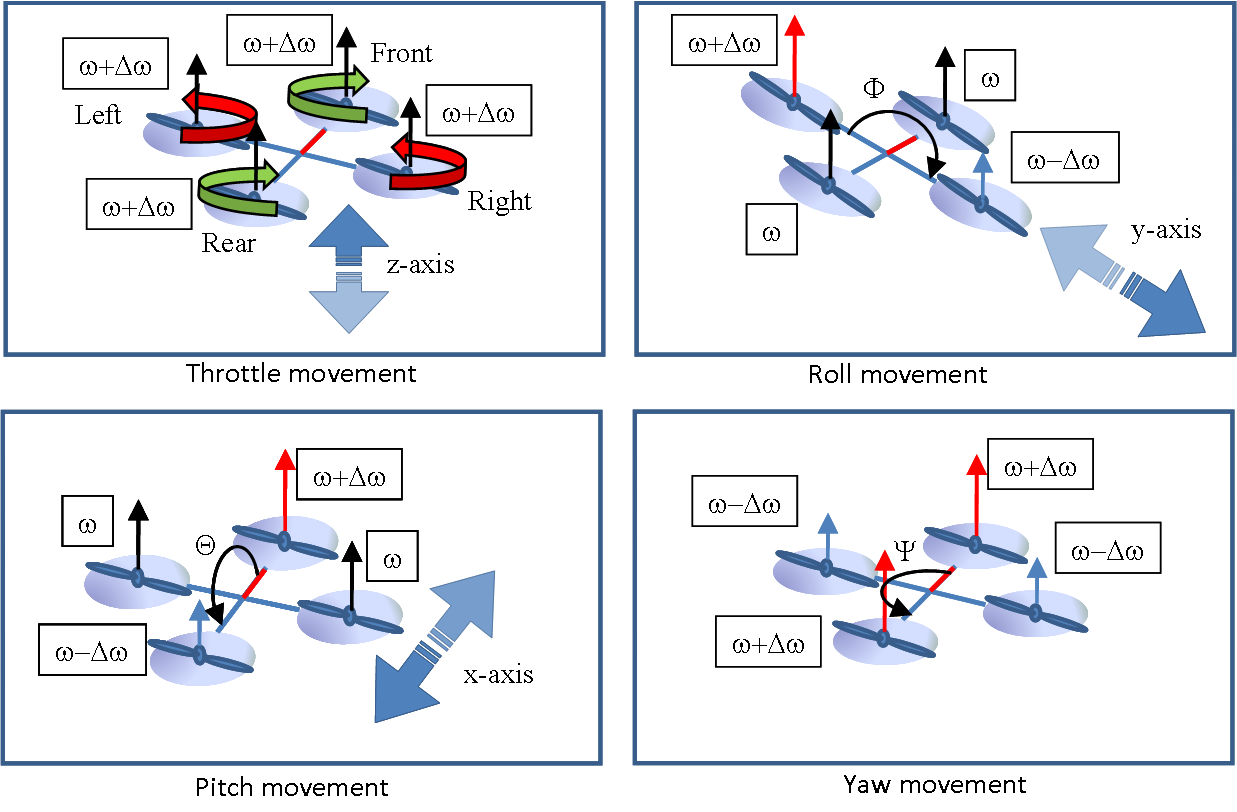
\includegraphics[width=1\textwidth]{graphic/QuadrotoDOF.png}
	\caption{Degrees of Freedom of a quadrocopter}
	\label{fig:quadrotoDOF}
\end{figure}


To keep the equilibrium of rotational kinematics and to prevent self-rotation,
the motor direction of rotation equals crosswise. The quadrocopter has six \gls{DOF}
~ which can be distinguished as angular and translational movements.
Translational movements can be executed in x-, y- and z- axis.
 Accelerating all rotors with the same speed \gls{sym_omega} to the value
 of \gls{sym_delta_omega} will affect a throttle movement \gls{sym_U_1}~[N] in z-direction.
Movements to the negative direction of the z-axis are possible, if the summarised thrust of
the four rotors is smaller as the gravitational force of the aerial vehicle. The roll movement \gls{sym_U_2}~[N m]
 can be described as a change of the angle around the x-axis.
\newpage
Thereby the left and right rotors execute a force difference by slowing down
the one and simultaneous increasing the other speed with
\gls{sym_delta_omega}. 
Related to the thrust difference and angular
 movement, the aerial vehicle creates a force in the direction of the y-axis. Equivalent to roll,
 the pitch movement \gls{sym_U_3}~[N m] is executed with a change of the angle around the y-axis.
 Also the pitch movement creates a translational
movement across the x-axis. Pitch and roll can only reach a stable angular state
and accelerate to the x- or y-axis, if the value of
\gls{sym_delta_omega} 
is the same at the diagonal rotors. Otherwise, the quadrocopter would pure rotate
across the corresponding axis. The yaw movement \gls{sym_U_4}~[N m] is a rotation around the z-axis.
This angular movement results in combination of pairwise different thrusts and
takes as long as these thrusts are different \footnote{The theory and the identifiers of this chapter bases on \citeref[pp.8-11 Quadrotor model and system]{Bre08}}.


\subsection{Equations of Motion} %5 Seiten (act sum 7) (Try to reduce this chapter)
\label{mt:c:literature:s:equations_of_motion}

Simulations of dynamic systems are based on physical models which describe their
motion. So the behaviour of the quadrocopter also can be described by using \gls{EOM},
\gls{WRT}~ the input parameters of the model. Thanks to these equations, it is viable
to predict and define the positions, velocities and accelerations of the
quadrocopter by investigating the four motor speeds. Bouabdallah 
\citeref[pp.15-24 System Modelling]{Bou07} demonstrates two methodologies to
derive the \gls{EOM}~ with the Newton-Euler and Euler-Lagrange formalism.
\newpage 
The Euler-Lagrange formalism derives the \gls{EOM}~ by calculating the difference of the
kinetic and potential energy of the system under consideration of the general coordinates and forces 
\footnote{See \citeref[pp. 218-219 The Lagrangian Method]{Mor07}}.
The Newton-Euler formalism bases on the Newton-Euler equations
\citeref[p.106 The original recursive Newton-Euler equations]{Fea08} which
describe the combined translational and rotational dynamics of a rigid-body \gls{WRT} the centre of mass.
 Both formalisms follow different approaches to derive the \gls{EOM}, but are based
on the same coordinate systems. These two coordinate systems have different origins and describe
 movements from different perspectives. One coordinate system can be considered as observer perspective to
 the quadrocopter because it describes the absolute position in space and is
 called earth inertial frame (E-frame). 

In contrast to that, the second
 coordinate system is a body fixed frame (B-frame) and is defined as system of
 relative movements which originates in the middle of the symmetric rigid
 quadrocopter body
\footnote{An origin which is coincidence to the centre of mass simplifies the
 Newton-Euler equation enormous, See \citeref[p.98 The original recursive
 Newton-Euler equations]{Fea08}}. Bresciani \citeref[pp.8-23 Quadrotor model and
 system]{Bre08} shows in his
work the identification and derivation of the \gls{EOM}~ by using the Euler-Newton
formalism and gives reasons why \gls{EOM}~ are more conveniently formulated in the
B-frame or further in a mixture called hybrid frame (H-frame) \footnote{See
\citeref[p.19 Hybrid frame]{Bre08} }. A part of these congenial reasons focus the
simplicity to convert on-board measurements to the B-frame coordinates and the
matter of fact that the control  forces almost are given in B-frame.
The other part describes simplifications in
 the mathematical derivation causes of B-frames symmetrical behaviour and the time
 invariance of the inertias
\footnote{See \citeref[p.12 Conveniently formulated \gls{EOM}]{Bre08} }.
\newpage
In the following figures\footnote{This picture
extends the coordinate system picture presented in\citeref[p.20 OS4 coordinate
system]{Bou07}}, we can see the both coordinate systems and the movements in the
\gls{DOF}~ which are interesting.



\begin{figure}[H]
	\centering
		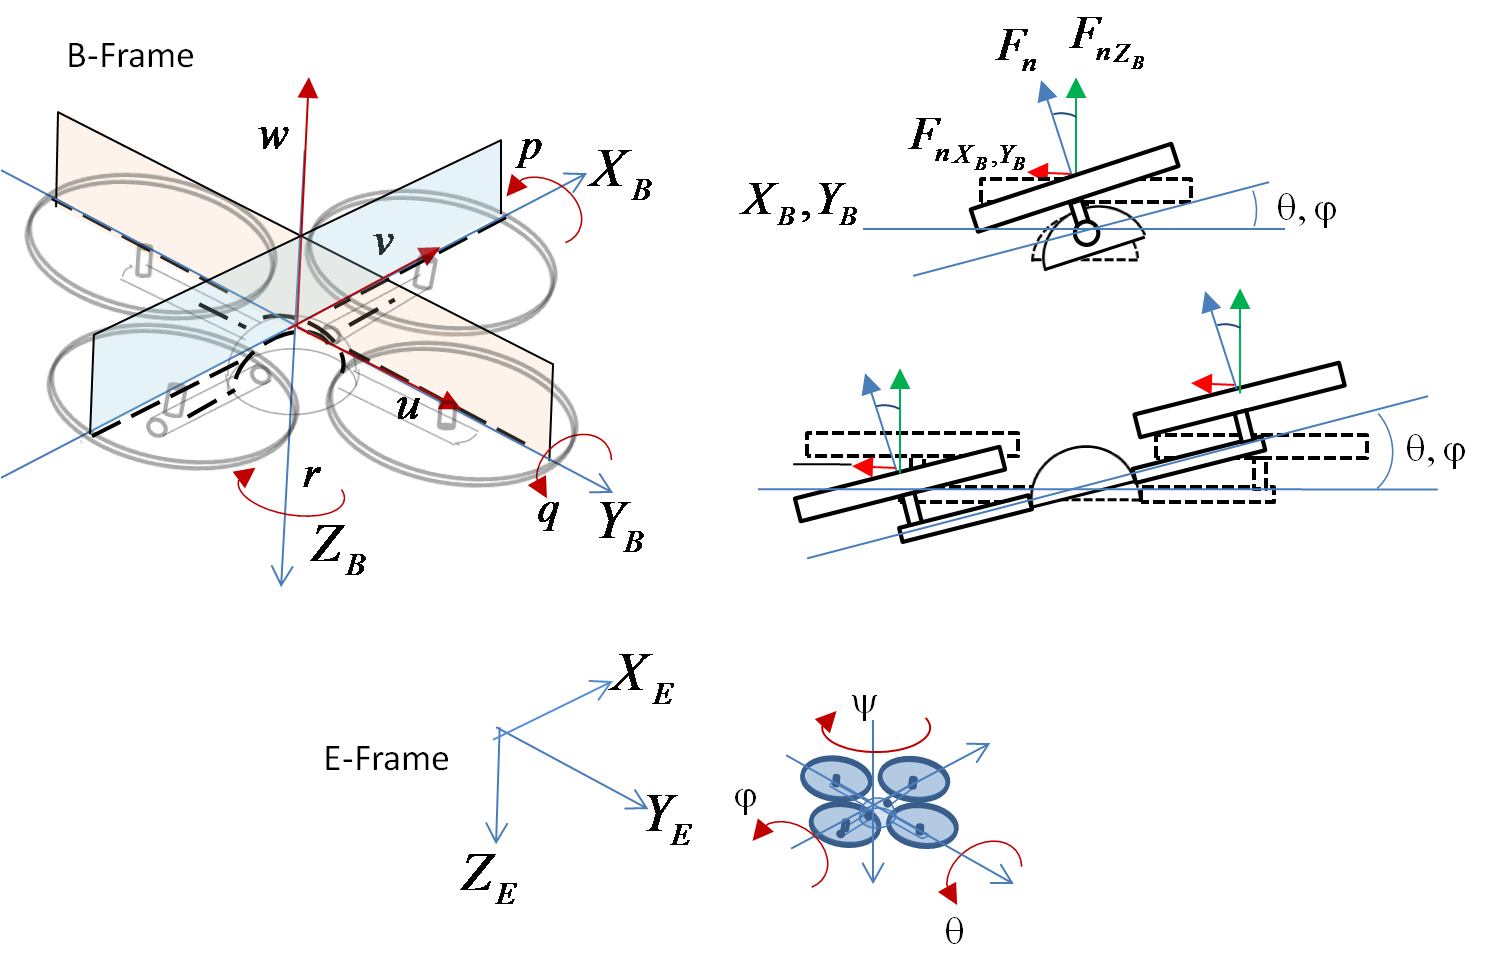
\includegraphics[width=1\textwidth]{graphic/QuadrocopterPhysicalModel.png}
	\caption{Quadrocopter movements and coordinate systems}
	\label{fig:QuadrocopterPhysicalModel}
\end{figure}

The starting point of Brescianis derivation is to define an equation, which
describe a generic 6 \gls{DOF}~ rigid-body (See \ref{formula:eom_dot_xi}) with the
\gls{GVV}~ \gls{sym_dot_xi} \gls{WRT}~ the E-frame, the \gls{GVV} \gls{sym_nu}~ \gls{WRT}~ the
B-frame and the generalized matrix \gls{sym_J_Theta} which includes the
rotation and the translation submatrix \gls{sym_R_Theta},
\gls{sym_T_Theta} which transforms \gls{sym_nu} to
\gls{sym_dot_xi} (See \ref{formula:eom_J_Theta} ). The definition of the \gls{GVV}~
and the \gls{GPV}~ \gls{WRT}~ the corresponding frames are visualized in figure
\ref{fig:QuadrocopterPhysicalModel}
 and can be described with the equations \ref{formula:eom_nu} and
 \ref{formula:eom_xi}. Thereby \gls{sym_xi} is composed of the linear
 position vector \gls{sym_Gamma_E}~ \lbrack m\rbrack~ and the angular
 position vector \gls{sym_Theta_E}~ \lbrack rad\rbrack. Similar to the
 position vector, the velocity vector is composed of a linear velocity vector
 \gls{sym_V_B}
~\lbrack m/s\rbrack~ and an angular velocity vector \gls{sym_omega_B}
 ~\lbrack rad/sec\rbrack. 
\newpage
The essence frame of interest is a mixture of the both
 mentioned frames, called H-frame, which contains the linear velocity vector
 \gls{sym_dot_Gamma_E}~\lbrack m/s\rbrack~ from E-frame and the angular
 velocity vector \gls{sym_omega_B}~\lbrack rad/s\rbrack~ from B-frame
 \ref{formula:eom_zeta}. Brescianis interest was to define a frame which can be
 transferred to an acceleration vector ~\gls{WRT}~ the H-frame and to facilitate the
 ~\gls{EOM}~ under consideration of typical ~\gls{IMU}~ values of a quadrocopter.
% (Write to Appendix the derivations and the complete Matrixes \R_{\Theta} and
% \T_{\Theta}).

Bresciani uses the Euler-Newton equations (See
\ref{formula:eom_F_B_tau_B})\footnote{See \citeref[p.13 The dynamics of a generic
6 DOF rigid-body]{Bre08}} to derive the matrix form which is composed
 of the system inertia matrix \gls{sym_M_B} and a Coriolis-centripetal
 matrix \gls{sym_C_B_nu}. A ~6 \gls{DOF}~ rigid-body dynamics system inertia
 matrix takes the mass of the body \gls{sym_m} \footnote{The notation \ensuremath{I_{3x3}}
 means 3 times 3 identity matrix (See \gls{sym_I_nxn})} ~\lbrack kg\rbrack~ and its inertia \gls{sym_I} ~\lbrack
 \ensuremath{Nms^2}\rbrack~ into account.

% (Write Calculation to Appendix).
 Furthermore Bresciani recognized that the quadrocopter dynamics can be divided
 to three contributors which describe the gravitational vector
 \gls{sym_G_B_xi} \footnote{\gls{sym_G_B_xi} considers the acceleration
 of gravity g ~\lbrack \ensuremath{m/s^2}\rbrack~ and influences the linear
 forces, See \citeref[p.15 The gravitational vector]{Bre08}}, the gyroscopic
 torque \gls{sym_O_B_nu}*\gls{sym_Omega}\footnote{\gls{sym_O_B_nu}*\gls{sym_Omega} considers the gyroscopic
 effects of the propeller rotation which influence the angular forces. Thereby
 \gls{sym_O_B_nu} is the propeller matrix and \gls{sym_Omega}~
 \lbrack\ensuremath{rad/s}\rbrack~ the proppelers' speed vector See \citeref[p.16
 The gyroscopic torque]{Bre08}} and the movement vector with the inputs of the
 system \gls{sym_E_B}\ensuremath{*}\gls{sym_Omega}\ensuremath{^2}(See \ref{formula:eom_F_B_tau_B}) \footnote{The
 constant matrix \gls{sym_E_B} \ref{formula:EB_Omega2} includes the thrust \gls{sym_b}
 \lbrack\ensuremath{Ns^2}\rbrack, \gls{sym_d}\lbrack\ensuremath{Nms^2}\rbrack and \gls{sym_l}l
 [m] (distance between the center of the quadrocopter and the
and the center of a propeller) factors of the input system. The inputs are given
with \gls{sym_Omega}\ensuremath{^2} because the forces and torques are proportional to the
squared propellers' speed, See
 \citeref[pp.129-135 Aerodynamics calculation]{Bre08}}.
 So it is possible to
 create a relation between the Newton-Euler equations (See
 \ref{formula:eom_F_B_tau_B}) and the sum of these three contributors
 (\ref{formula:eom_F_B_tau_B}), to isolate the \gls{GAV} \gls{sym_dot_nu}, and to
 derive the ~\gls{EOM}~ \gls{WRT}~ the B-frame (See \ref{formula:eom_dot_nu}).
\newpage 
Equivalent to that, the substitution of ~\gls{GAV}~ \gls{sym_dot_nu} with \gls{GAV}
 \gls{sym_dot_zeta} ~\gls{WRT}~ the H-frame in
 \ref{formula:eom_dot_zeta_unsolved}, gives an equation which can be
solved to \gls{sym_dot_zeta} for the determination of the required ~\gls{EOM}~
and a quadrocopter model with typical ~\gls{IMU}~ values (See
\ref{formula:eom_dot_zeta_solved}).

\tikzstyle{block}=[rectangle,
 %draw=black,
 %rounded corners,
 %fill=blue!20,
 text centered,
 text=black, text width = 4cm, anchor=east]

\tikzstyle{refLabel}=[rectangle, anchor=east]
 
% \linespread{0,8}

\begin{tikzpicture}[remember picture]

%       (5,10)
%(0,8)  (5,8)  (10,8)
%       (5,6)
%       (5,4)
%(0,2)          (10,2)
%(0,0)


\node [block, text width = 4cm] (_5_10) at (0.6,11.6) {\begin{equation}
\begin{split}
\label{formula:eom_dot_xi}
\small\dot\xi=J_\Theta*\nu
\end{split}
\end{equation}
};

\node [block, text width = 5.5cm] (_0_8) at (-2.6,7.4) {\begin{equation}
\begin{split}
\label{formula:eom_xi}
\small \xi=
\begin{pmatrix} \Gamma^E \\ \Theta^E \end{pmatrix}=
\small\begin{pmatrix} x_e \\ y_e \\ z_e \\ \phi \\ \theta \\ \psi \end{pmatrix}
\end{split}
\end{equation}
};

\node [block, text width = 5.5cm] (_5_8) at (1.2,9) {
\begin{equation}
\begin{split}
\label{formula:eom_J_Theta}
\small  J_\Theta=\begin{pmatrix} R_\Theta & 0_{3x3} \\ 0_{3x3} & T_\Theta\\
\end{pmatrix}
\end{split}
\end{equation}
};

\node [block, text width = 5.5cm] (_10_8) at (4.2,7.4) {
\begin{equation}
\begin{split}
\label{formula:eom_nu}
\small \nu = 
\begin{pmatrix} V^B \\ \omega^B\end{pmatrix} =
\begin{pmatrix} u \\ v \\ w \\ p \\ q \\ r \end{pmatrix} 
\end{split}
\end{equation}};

\node [block, text width = 5.5cm] (_5_6) at (1,4) {
\begin{equation}
\begin{split}
\label{formula:eom_zeta}
\small \zeta = 
\begin{pmatrix} \dot\Gamma^E \\ \omega^B\end{pmatrix} =
\begin{pmatrix} \dot x_e\\ \dot y_e \\ \dot z_e\\ p \\ q \\ r \end{pmatrix}
\end{split}
\end{equation}};

\node [block, text width = 12cm] (_5_4) at (4.4,0.2) {
\begin{equation}
\begin{split}
\label{formula:eom_F_B_tau_B}
\small
\begin{pmatrix} F^B \\ \tau^B \end{pmatrix} =
\begin{pmatrix} m*I_{3x3} & 0_{3x3} \\ 0_{3x3} & I \end{pmatrix}
\begin{pmatrix} \dot V^B \\ \dot \omega^B \end{pmatrix} + 
\begin{pmatrix} \omega^B \times (m*V^B) \\ \omega^B \times (I*\omega^B) \end{pmatrix}\\ =
 M_B*\dot\nu + C_B(\nu)*\nu=G_B(\xi)+O_B(\nu)*\Omega+E_B*\Omega^2
 \end{split}
 \end{equation}};

\node [block, text width = 11.5cm] (_0_2) at (4.4,-2.4) {
\begin{equation}
\begin{split}
\label{formula:eom_dot_zeta_unsolved}
\small 
M_H*\dot\zeta+C_{H}(\zeta)*\zeta=G_H+O_{H}(\zeta)*\Omega+E_{H}(\xi)*\Omega^2
\end{split}
\end{equation}
};
\node [block, text width = 11cm] (_10_2) at (4.4,-3.6) {\begin{equation}
\label{formula:eom_dot_nu}
\small \dot\nu=M_B^{-1}*(-C_{B}(\nu)*\nu+G_B(\xi)+O_B(\nu)*\Omega+E_B*\Omega^2)
\end{equation}};

\node [block, text width = 11cm] (_0_0) at (4.4,-4.6) {\begin{equation}
\label{formula:eom_dot_zeta_solved}
\small 
\dot\zeta=M_H^{-1}*(-C_H(\zeta)*\zeta+G_H+O_H(\zeta)*\Omega+E_H(\xi)*\Omega^2) \end{equation}};

% \path[->] (_5_10) edge[thick] (_0_8);
% \path[->] (_5_10) edge[thick] (_5_8);
% \path[->] (_5_10) edge[thick] (_10_8);
% 
% \path[->] (_0_8) edge[thick, bend right=30] (_5_6);
% \path[->] (_0_8) edge[thick, bend right=30] (_5_4);
% 
% \path[->] (_10_8) edge[thick, bend left=30] (_5_6);
% \path[->] (_10_8) edge[thick, bend left=30] (_5_4);
% 
% \path[->] (_5_6) edge[thick, bend right=85] (_0_2);
% % \path[->] (_5_4) edge[thick] (_0_2);
% \path[->] (_5_4) edge[thick] (_10_2);
% 
% \path[->] (_0_2) edge[thick] (_0_0);
% 



\draw[thick,-<](-1.4,10.6) .. controls (-1.4,9.4) and (-1.4,9.4) .. (-1.4,9.6);

\draw[thick,->, dashed](-4.4,3.6) -- (-7.6,3.6) -- (-7.6,-1) -- (-6,-2.2);
\draw[thick,->](-3.2,11) -- (-4.2,9.6);
\draw[thick,->](1,11) -- (2,9.6);
\draw[thick,->](-5,4.2) -- (-5,2.2);
\draw[thick,->](2,4.2) -- (2,2.2);
\draw[thick,->](-6.8,-3) -- (-7.4,-3) -- (-7.4,-5.2) -- (-6.8,-5.2);
\draw[thick,->](-3.6,6) -- (-2.6,5.2);
\draw[thick,->](0.6,6.2) -- (-0.4,5.2);
\draw[thick,->](4.6,0.6) -- (5.4,0.6) -- (5.4,-2.6) -- (4.6,-2.6);
\draw[thick,->](4.6,1) -- (6,1) -- (6,-3.8) -- (4.6,-3.8);
\end{tikzpicture}


%-----------------------------------------------------------------------------------
%\begin{figure}[H]
%	\centering
%		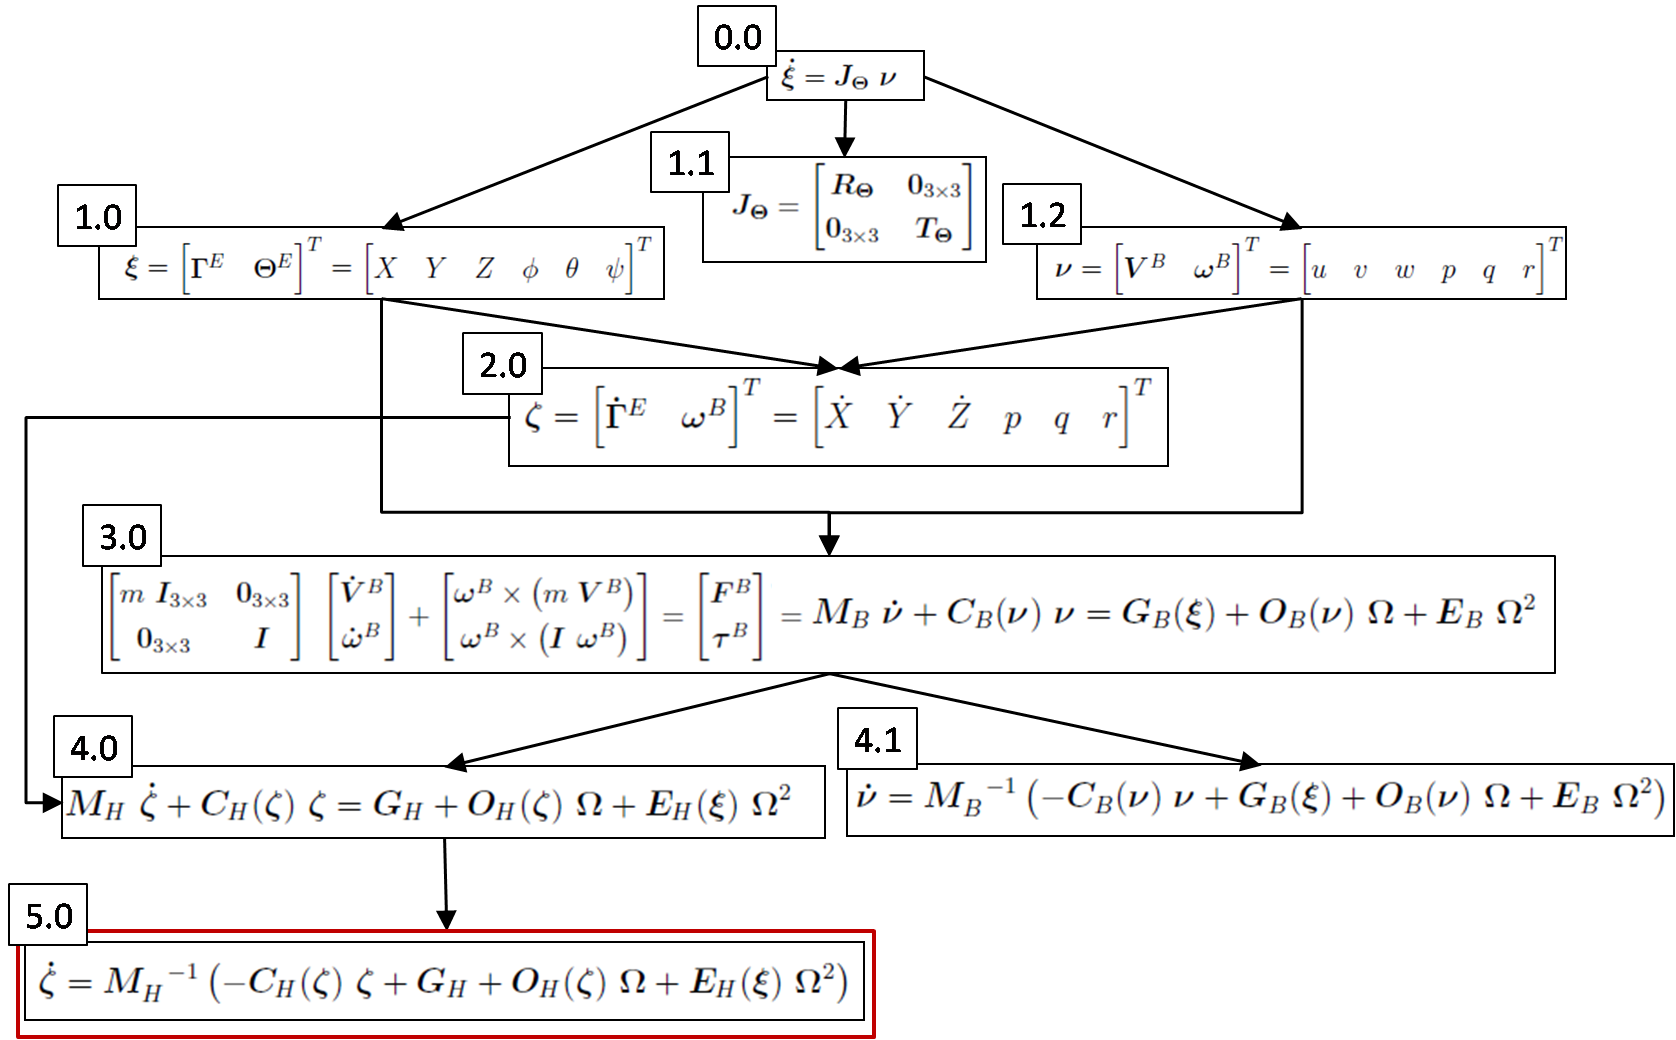
\includegraphics[width=0.75\textwidth]{graphic/BrescianiDerivation.png}
%	\caption{Derivation of GAV WRT the B and H-frame }
%	\label{fig:QuadrocopterPhysicalModel}
%\end{figure}
%-----------------------------------------------------------------------------------
\newpage
The following equations show the derived ~\gls{EOM}~ of the ~\gls{GAV}~
\ensuremath{\dot\zeta} ~\gls{WRT}~ the H-frame. Apparent from the rotational ~\gls{DOF}~
of the quadrocopter, the linear accelerations ~\ensuremath{\dot\Gamma^E} ~\gls{WRT}~
the E-frame are influenced by a trigonometrical equation of the angles
~\gls{sym_Theta_E} and the sum of the uplift forces
~\gls{sym_U_1}. This behaviour is also visualized in the
cross-sectional and front side view ~\gls{WRT}~ the specific angle and B-frame axis
in the figure \ref{fig:QuadrocopterPhysicalModel}. Further the equations show
the angular accelerations \ensuremath{\dot\omega^B}~ \gls{WRT}~ the B-frame and the
corresponding influences which derive from the propellers' force constellation
\gls{sym_U_1}, \gls{sym_U_2}, \gls{sym_U_3}, \gls{sym_U_4}(See chapter \ref{mt:c:LiteratureReview:QuadrocopterFlightDynamics})
, the angular velocities from
\ensuremath{\omega^B} and the body inertias ~\gls{WRT}~ the mass axis 
\footnote{The formula \ref{formula:dot_zeta} bases on \citeref[p.21 The GAV WRT H-frame]{Bre08}}
\footnote{\ensuremath{J_{TP}}~ \lbrack N m s2\rbrack~ is the total rotational moment of inertia around the propeller axis, 
See \citeref[p.16 Propeller inertia]{Bre08}}
\footnote{\ensuremath{I_{XX}, I_{YY}, I_{ZZ}}~ \lbrack kg m2\rbrack~ are moments
of inertias around the specific axis, 
See \citeref[p.136 Inertia matrix]{Bre08}}
\footnote{The identifiers of this chapter are derived from \citebib{Bre08}}.



\begin{equation}
\label{formula:dot_zeta}
\linespread{0,8}
\ensuremath{\dot\zeta} = \begin{pmatrix} \ddot x_e \\ \ddot y_e \\ \ddot
z_e \\ \dot p \\ \dot q \\ \dot r \\\end{pmatrix}
=
\begin{pmatrix}
  (sin\psi sin\phi
  +cos\psi sin\theta cos\phi)\frac{U_1}{m} \\
  (-cos\psi sin\phi + sin\psi sin\theta cos\phi)\frac{U_1}{m} \\
  -g+(cos\theta cos\phi)\frac{U_1}{m} \\

  \frac{I_{YY}-I_{ZZ}}{I_{XX}}qr -\frac{J_{TP}}{I_{XX}}q\Omega+\frac{U_2}{I_{XX}}\\

  \frac{I_{ZZ}-I_{XX}}{I_{YY}}pr +\frac{J_{TP}}{I_{YY}}p\Omega+\frac{U_3}{I_{YY}} \\

   \frac{I_{XX}-I_{YY}}{I_{ZZ}}pq+\frac{U_4}{I_{ZZ}} \\
\end{pmatrix}
\end{equation} 

\begin{equation}
\label{formula:EB_Omega2}
U_B=E_B\Omega^2=
\begin{pmatrix} 0\\ 0\\ U_1 \\ U_2 \\ U_3 \\ U_4\end{pmatrix}=
\begin{pmatrix}
0\\
0\\
b(\Omega_1^2+\Omega_2^2+\Omega_3^2+\Omega_4^2) \\
l b(-\Omega_2^2+\Omega_4^2) \\
l b(-\Omega_1^2+\Omega_3^2) \\
d(-\Omega_1^2+\Omega_2^2-\Omega_3^2+\Omega_4^2)
\end{pmatrix}
\end{equation}
\section{Vision-based Sensors} % 5 Seiten (act sum 13)
This chapter introduces why visual sensors are interesting in actual technological developments of \gls{UAV} systems, which approaches exist and what the benefits and drawbacks are. The mentioned approaches are separated thereby in several domains and compared with each other.
The outcomes of this review about vision-based sensors and the related topics, include some decision criteria of the realised approach in focus of this project.
  

\subsection{Motivation}
An enormous quantity of researches, which is sponsored by industry companies and
universities, was executed to find a better approach to stabilize ~\gls{UAV}~ by
using different sensors. Movement detection approaches, which are ultrasonic, sonar or
~\gls{RF}~ based show that it is necessary to have known reference points to get a
reliable result  \citebib[p.2 Ultrasound indoor localization with reference
points] {EckDreGer09}\citeref[pp.4-5 Radio Model Localization]{BulHeiEst02}. The
problem of these approaches is that the environment has to be prepared before the
\gls{UAV} flight. This preparation is a drawback in point of flexibility in different
operation places. Anyway, approaches with ultrasonic, ~\gls{RF}~ or sonar sensors
show that the localization of ~\gls{UAV}~ needs a kind of global feedback to correct
the ~\gls{UAV}~ absolute position. One of the first motivations for a vision-based
sensor was presented by Ettlinger et al. \citeref[pp.1-2 Visual-Based Localization and
Control]{EttNecIfjWas04}.
\newpage
In this paper, the authors suggest that vision is the
only practical solution for obstacles of reference free flight stability, and
showed an On-board approach for a ~\gls{GUAV}~ by detecting the horizon with a
forward looking camera and estimating and control the flight attitude\citeref[p.27 Vision
Sensors]{Tip08}.
The intension of a reference free vision-based stability
approach, for solving the ~\gls{IMU}~ error drift, is the motivation for the
investigation of visual approaches, which will be introduced and compared in this chapter.


\subsection{Distribution and Implementation Approaches}
\label{mt:c:LiteratureReview:Distribution and implementation approaches}

This chapter focus the comparison of different approaches of vision sensors'
implementations and distributions, which were researched in several scientific
works. These approaches are separated in distribution approaches (\gls{OFIP},~
\gls{ONIP},~ \gls{ONCA},~ 
\gls{OFCA}), as visualized in figure
\ref{fig:Off-vsOn-BoardCamerasIp.png}, and the implementation approaches
\gls{HWBIP}~ and \gls{SWBIP}. Problems, such as a limited power resource, a poor level of
algorithm complexity for \gls{ONIP}~ resulting from the limited calculating On-Board
performance and the endeavour to economise weight, lead to outsourcing the image
processing to a remote system via a wireless communication, which is not
concerned to the On-Board problems. A drawback of this approach was examined by
Langer et al. \citeref[pp.5-7 Off-Board Image Processing]{LanSuePro08} which use
\gls{OFIP}~ to track a landing pad for autonomous landing and show that the wireless
transmission delay has a impact on the sampling rate of the algorithm.\newpage
Tippetts \citeref[p.27 Vision Sensors]{Tip08} mentions in his work the limitation of the
wireless communication in \gls{OFIP}~ as a drawback for range of the aircraft
\footnote{The comparison of \gls{OFIP}~ and \gls{ONIP}~ approaches is visualized in 
\ref{fig:ComparisonVisualApproaches.png}}. 
The \gls{OFCA}~ approach was researched by
Altug et al. \citeref[p.76 Localization and Control with an Off-Board
camera]{AltOstMah02}, with the result of a less sensitive feature detection and
position localization compared to the \gls{ONCA}~ approach. \gls{OFCA}~ tracking is shown in
the developments of extremely reliable and precise localization of a \gls{UAV}~ and
is used in the development of aggressive autonomous flights of multiple \gls{MAV}~ in
the experiments of Mellinger et al. \citeref[Trajectory Generation and Control with
Off-Board cameras] {MelMicKum10} \citebib[pp.363-364]{GurStuAchDotHirRus07}.

\begin{figure}[H]
	\centering
		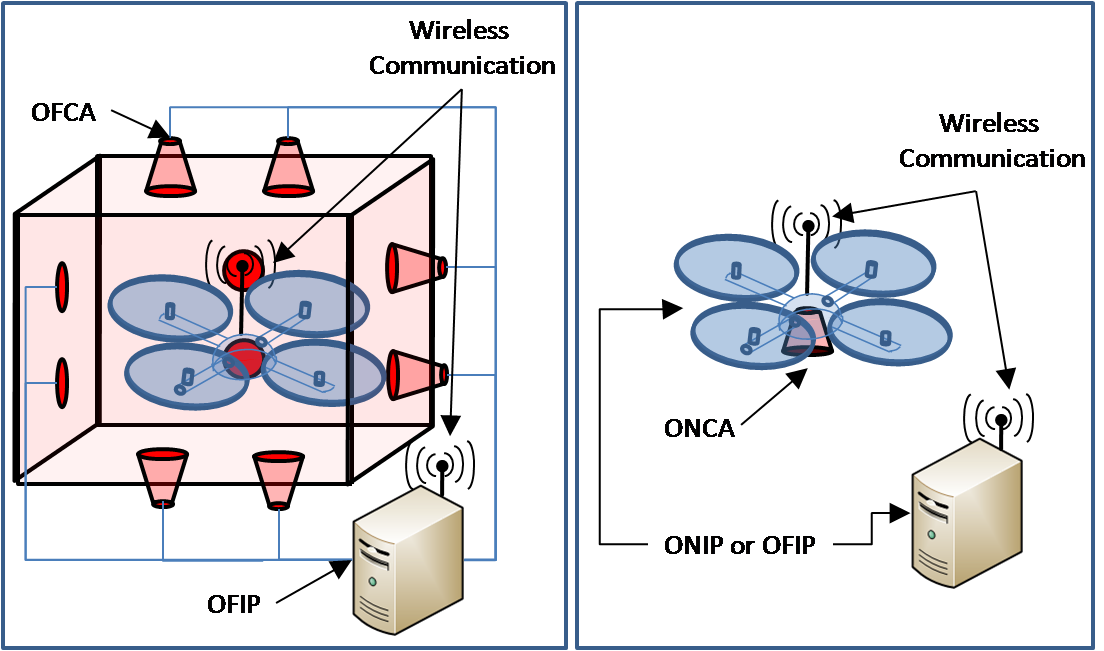
\includegraphics[width=1\textwidth]{graphic/Off-vsOn-BoardCamerasIp.png}
	\caption{On- and Off-Board camera and motion tracking system approach}
	\label{fig:Off-vsOn-BoardCamerasIp.png}
\end{figure}

% HW-based image processing
The advantage of \gls{OFCA}~ tracking system is that the image capturing and position
tracking is executed outside the \gls{UAV}~ and prevents complex On-Board
calculations for movement and position estimation \footnote{This approach focus the E-frame
localisation and is robust against position drifts and errors}.
\newpage
The disadvantage of this \gls{OFCA}~ method is that they need a special flying environment, which is
build up with an \gls{OFCA}~ motion tracking system\footnote{The comparison of \gls{OFCA}
and \gls{ONCA} approaches is visualized in \ref{fig:ComparisonVisualApproaches.png}}
\citebib[pp.1-2 The GRASP Testbed]{MicMelLinKum10}. Tippetts \citeref[pp.21-22 On-Board image processing with an FPGA] {Tip08}
realised an \gls{ONIP}~ approach with a \gls{FPGA},~which uses a complex feature tracking
algorithm, but runs with high sampling rate \footnote{In this case a high sampling
rate means that the image processing runs nearly equal to the sampling rate of
the \gls{IMU}}. 

The characteristics of the feature tracking with a \gls{FPGA}~ can result
a fast movement tracking method, but it is not an efficient method in the focus
of power consumption because the hardware is not optimised for the image
processing tasks.
In contrast to the drawbacks of \gls{FPGA}, Langer et al. \citeref[On-Board image
processing with mice sensors]{LanSuePro09} and Beyeler et al.
\citeref[pp.4-5]{BeyChrFlo09} showed an approach for detecting the spatial
movement of a \gls{UAV}~ with optical mice sensors, which have an optimized  hardware
for image processing and are lightweight.

These sensors calculate the optical
flow of the captured images and estimate the movement direction of the \gls{UAV}~ in
hardware and can provide a high sample rate. In contrast to the fast movement
detection, a disadvantage is that these sensors have limitations related to the
operating environments. These limitations are the concrete light and distance
range which is required from the manufacturer \citebib[pp.7-15 Limitations of the
operating environment] {ST05_1}\citebib [p.6 Performance of the optical flow
based position controller] {LanSuePro09}

% SW-based image processing
 \gls{SWBIP}~ approaches have a more flexible extension and change behaviour for
 prototyping of vision-based solutions, but they don't work as fast as \gls{HWBIP}~
 approaches. 
\newpage
Stowers et al. \citeref{StoBaiHayMil09}realized a heading estimation for a quadrocopter with
 an onboard \gls{SBC}~ which runs the open source computer vision toolkit
 \gls{OpenCV} \citebib{OpenCV2_0}.
This software based image
 processing approach shows strengths in the modularity of the image processing
 architecture and in the interchangeability of the vision system\footnote{The
 comparison of \gls{HWBIP}~ and \gls{SWBIP}~ approaches is visualized in 
\ref{fig:ComparisonVisualApproaches.png}} \citebib [pp.1-6 Software Based Vision
 Processing] {StoBaiHayMil09}\citebib[Software Structure and
 Portability]{GarKae08}. Figure \ref{fig:ComparisonVisualApproaches.png} includes
 the summary of the examined approaches of this chapter. We can see that no
 approach has outstanding set of beneficial characteristics. Each approach
 brings advantages and disadvantages, so the decision of the appropriate
 approach relates to the focus of investigation.

\begin{figure}[H]
	\centering
		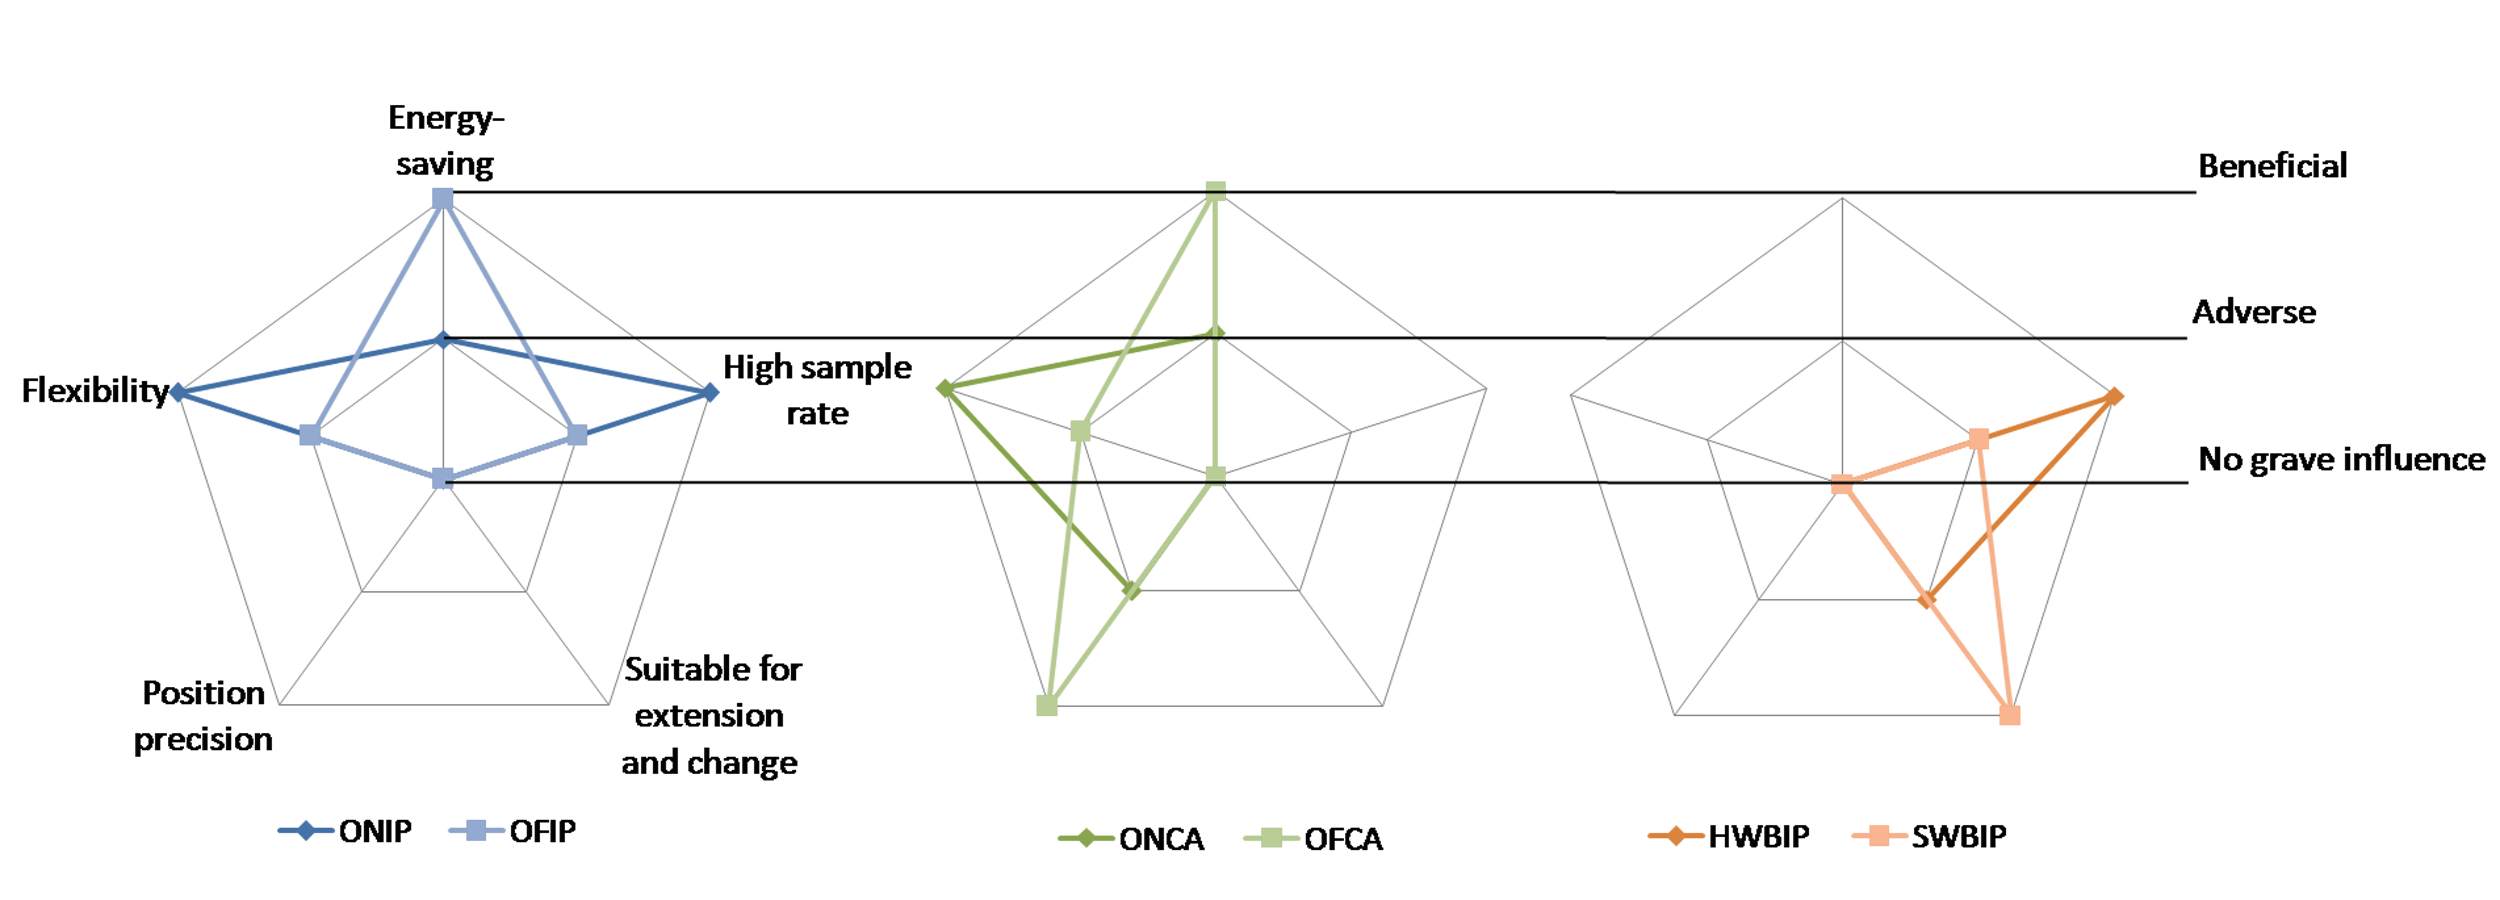
\includegraphics[width=1\textwidth]{graphic/ComparisonVisualApproaches2.png}
	\caption{A comparison of the distribution behaviour of vision sensors}
	\label{fig:ComparisonVisualApproaches.png}
\end{figure}

\subsection{Vision-based Movement Detection Algorithms} % 1 Seite vision-based movement detection algorithms

Sequential captured images contain a huge amount of information about the
absolute and relative movement of objects in every direction.
\newpage
So several vision-based movement detection approaches were researched in the topic of \gls{UAV}~
stability with different requirements to the information which extracted from the
vision process\footnote{These investigated approaches are visualized in figure
\ref{fig:VisualApproaches.png}. This figure includes pictures presented in
\citeref[SLAM]{Hay11}\citeref[Edge detector]{Koh11}\citeref[p.27 Horn and
Schunck optical flow]{BarFleBea94}}.
A simple approach for a relative vision
based control of a \gls{UAV}~ was implemented by Boabdallah \citeref[pp.110-114
Position Sensor]{Bou07} using a down looking camera and the Canny edge detector \citebib{Can86} and the Douglas Peuker Algorithm for curve equalisation \citebib{DouPeu73}. The drawback
of this approach is that the field of vision must contain forms with edges which
mean that the approach cannot result a satisfactory result if no edges are
detected. 

A further approach for detecting relative movements and to build up a
map for autonomous navigation, is visual \gls{SLAM}. This approach tracks features in
the field of vision and reconstructs the relation to the tracked features of previous
images. The realization of \gls{SLAM}~ \citebib{WilKleRei07} in a \gls{UAV}~ was executed
in the work of Bloesch et al. \citeref{BloWeiScaSie10} under consideration of
real-time characteristics. The behaviour of the algorithm shows that the
localization of the tracked features and the simultaneous mapping has a big
impact at the time delay of the calculation.

So the experiments and the control
algorithms were researched and designed for 7.5Hz sample rate. Another popular
tracking method for movement detection is given with the \gls{OF}, which can
be described as movement observation of tracked objects or pixels in a sequence
of images. Algorithms to calculate the \gls{OF} were introduced by Horn and
Schunk \citebib{HorSch80}, Lucas and Kanade \citebib{LucKan81}. A few
years after introducing the Lucas-Kanade-Algorithm, Lucas described the
theoretical approach of visual navigation by using the \gls{OF}. Thereby he
described the possibility to detect movements and to calculate correspondence
velocities.
\newpage
These velocities can be combined to a vector field which can describe
movements in every direction \citeref[pp.40-45 Optical Navigation Theory]{Luc84}.

\begin{figure}[H]
	\centering
		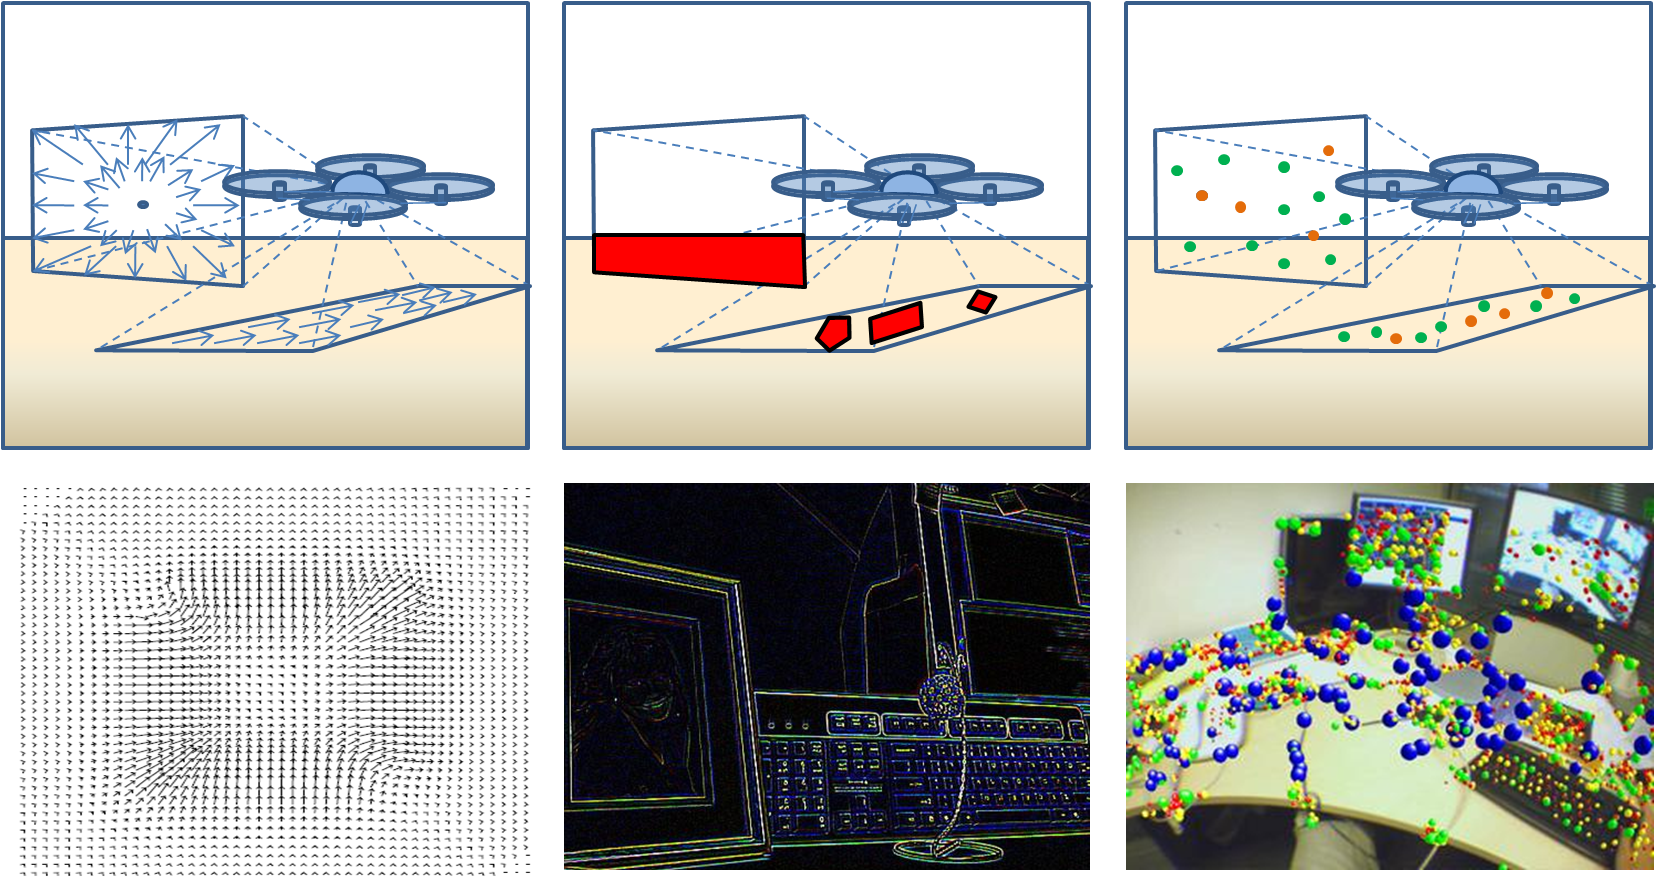
\includegraphics[width=1\textwidth]{graphic/VisualApproaches.png}
	\caption{Examples for UAV stabilisation with Optical Flow, Edge detection and SLAM}
	\label{fig:VisualApproaches.png}
\end{figure}

\subsection{Optical Flow}

Researches which are related to image processing, mostly use camera models to
reduce the complexity of the reality. This approach is also practicable in
researches with \gls{OF}. The figure \ref{fig:ProjectionModels.png}
visualizes a camera model with a spherical image plane, which illustrates a complex real
 camera and a flat image plane, that simplifies the complex model. Such
 simplification is achievable, if a mathematical transformation of the image plane
 can result a distortion-free image plane. Fach \citeref[pp.29-31 Chapter 3.3,
 Distortions]{Fac08} classifies reasons for distortions in a \gls{CACD}~ and the
 \gls{SOAD}. Pincushion- and barrel- distortions are summarized as radial distortions and
caused by focal distance in relation to the captured
image dimension. 
\newpage
Further decentering distortions are based on the wrong alignment
of the optical axis to the projected plane. 
Further Fach 
\citeref[pp.29-31 Matehmatical description of distortions]{Fac08} shows that these distortions of a
physical camera can be eliminated with the equations shown in appendix
\ref{mt:c:Appendix:Mathematical_description_of_distortions}. Thereby, the problem
of distortions is reduced to a factorisation of each distorted coordinate of the complete image.
 This process can be executed in the initial camera calibration
 phase, to eliminate distortions of the physical behaviour of the
lenses and the image plane of the camera, and further in situations in which the
camera is moved not planar to the projected plane. In the second case a fixed
\gls{IMU}~ of the camera system can provide the difference to the orthogonal gravity vector
g, and can allow the transformation of the captured image in real time
\footnote{Such a camera was introduced in the year 2009 as standalone system from
Fraunhofer Institute for Manufacturing Engineering and Automation ,See
\citeref[pp.1-2]{FraIpa09}}.

Following, the \gls{OF} projection suggested by Wei \citeref[pp.71-96
Obstacle Detection Using Optical Flow]{Wei09}, is described as a 2D-projection on the image plane
 of a 3D motion in the real world. Thereby Wei uses the ideal perspective
 projection model to introduce the projection of a
point \ensuremath{P=(X,Y,Z)}, from the camera frame into the image frame
\ensuremath{p=(x,y,f)} where f is the focal length. The \gls{OF} definition
is derived with the assumption that the point P moves in the time \ensuremath{t'}
to the Point \ensuremath{P'} with the corresponding projection on the image plane
p and \ensuremath{p'}.

The velocity on the image plane can be calculated as
\ensuremath{v=p-p'=(x, y, 0)^{T} - (x', y', 0)^{T}}, where the component of z is
cancelled out causing the 2D projection. Wei uses this projection to describe the problem
of retrieving the \gls{OF} velocity with 6 \gls{DOF}.
\newpage
Further Wei described that
researches, related to the \gls{OF} velocity determination, only can based on a reduced \gls{DOF}~
model\footnote{The \gls{DOF} of a ideal projection model are shown in figure
\ref{fig:ProjectionModels.png} The can be summarised in a translation vector
\ensuremath{T=(T_x, T_y, T_z)^{T}} and a rotational vector
\ensuremath{ \omega=(\omega_x, \omega_y, \omega_z)^{T}}, See
\citeref[pp.74-77 Motion Model Deduction]{Wei09}}.


\begin{figure}[H]
	\centering
		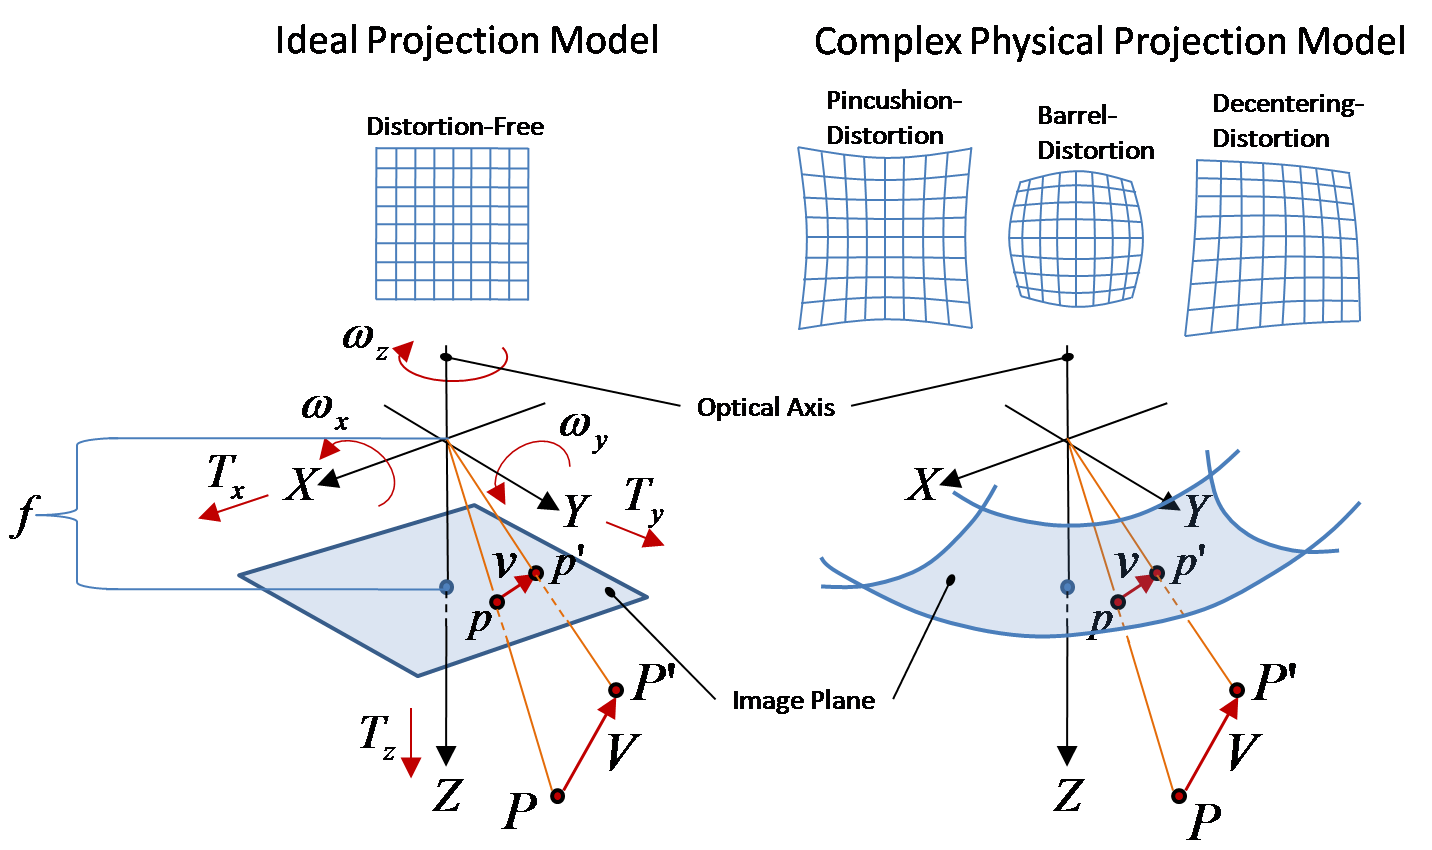
\includegraphics[width=1\textwidth]{graphic/ProjectionModels.png}
\caption{Complex Physical and Reduced Projection Camera Model}
	\label{fig:ProjectionModels.png}
\end{figure}

After introducing the projection camera models, the possibilities of \gls{OF} determination can be focused
with a top-down separation of algorithm classifications. These classification groups \gls{OF} algorithms to feature based, 
gradient based and correlation based methods. Feature based \gls{OF} algorithms usual execute three steps for the determination of the \gls{OF} field. At first, the images of a sequence are scanned for good features. Such features can be corners or regions of contrast peeks. Further found features are compared trough the image sequence with the result to determine for each step an \gls{OF} vector field. 
\newpage
The feature based \gls{OF} is robust against the aperture problem, which implies that just a part of the orthogonal movements can be detected in a image sequence with edges \citeref[p.24]{Tra10}. 

The figure \ref{fig:IntensitySample.png} 
\footnote{The presented image is downloaded from the website: http://www.1800skyride.com/} visualises the peeks of contrast regions. In this case the three hot-air balloons, in the square of the image, can be used as good features. Based on this example, the drawback of the feature based \gls{OF} is given in cases, if no features can be found.

\begin{figure}[!h]
	\centering
		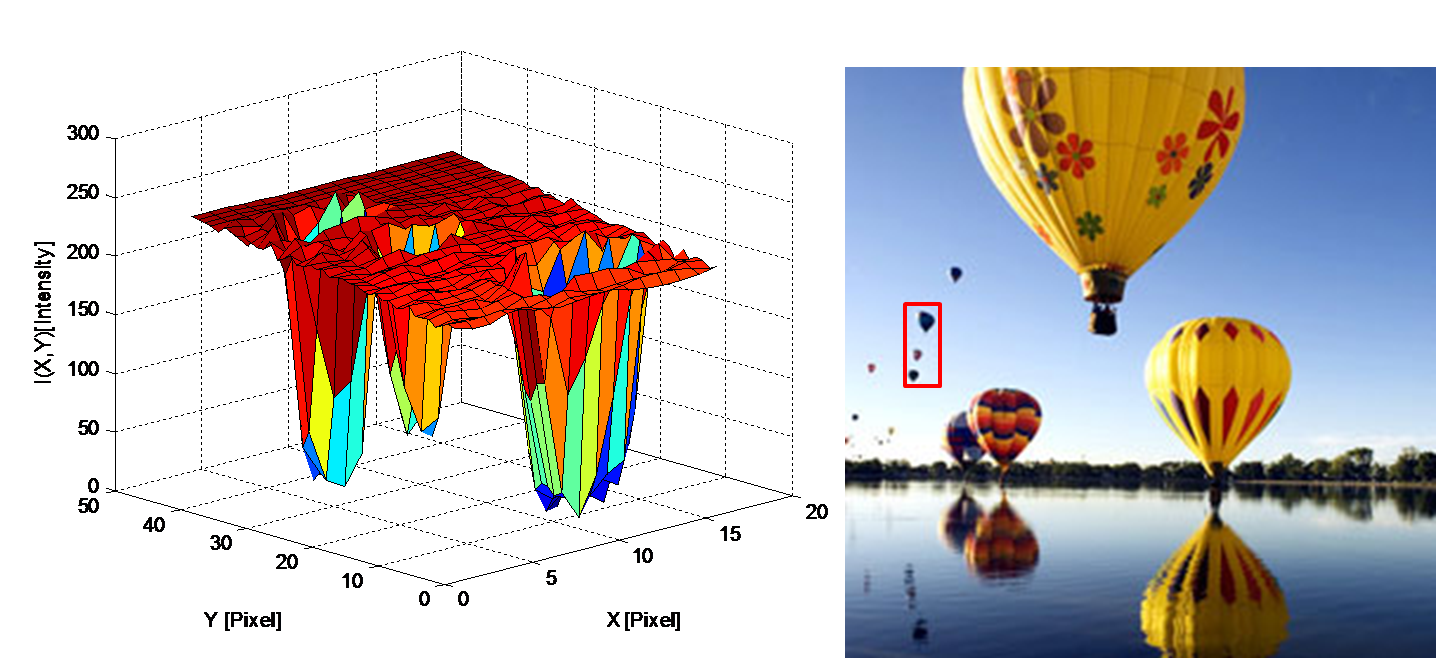
\includegraphics[width=1\textwidth]{graphic/IntensitySample.png}
\caption{Detected features visualised as peeks}
	\label{fig:IntensitySample.png}
\end{figure}

In contrast to that the gradient based algorithms can determine a optical flow field with no found features. This characteristic bases on the calculations of such algorithms, which use the intensity of images to determine the vector field. Thereby the movements of the intensities are determined with executing a minimising algorithm to the neighbourhood intensities. These determination is related to the disadvantage of intensive calculation complexity, which can be a drawback for real-time applications \citebib{HorSch80} \citebib{LucKan81}.
\newpage
An approach to improve the calculation complexity of the gradient based \gls{OF} determination, is given with the pyramids approach of Lucas and Kanade \citebib{LucKan81} (See figure \ref{fig:LucasKanadePyr.png}). The approach thereby downscales the pixel resolution with grouping pixels into blocks, with the average grayscale, and refines the image more and more until the intensity distances are determined satisfactory.

\begin{figure}[!h]
	\centering
		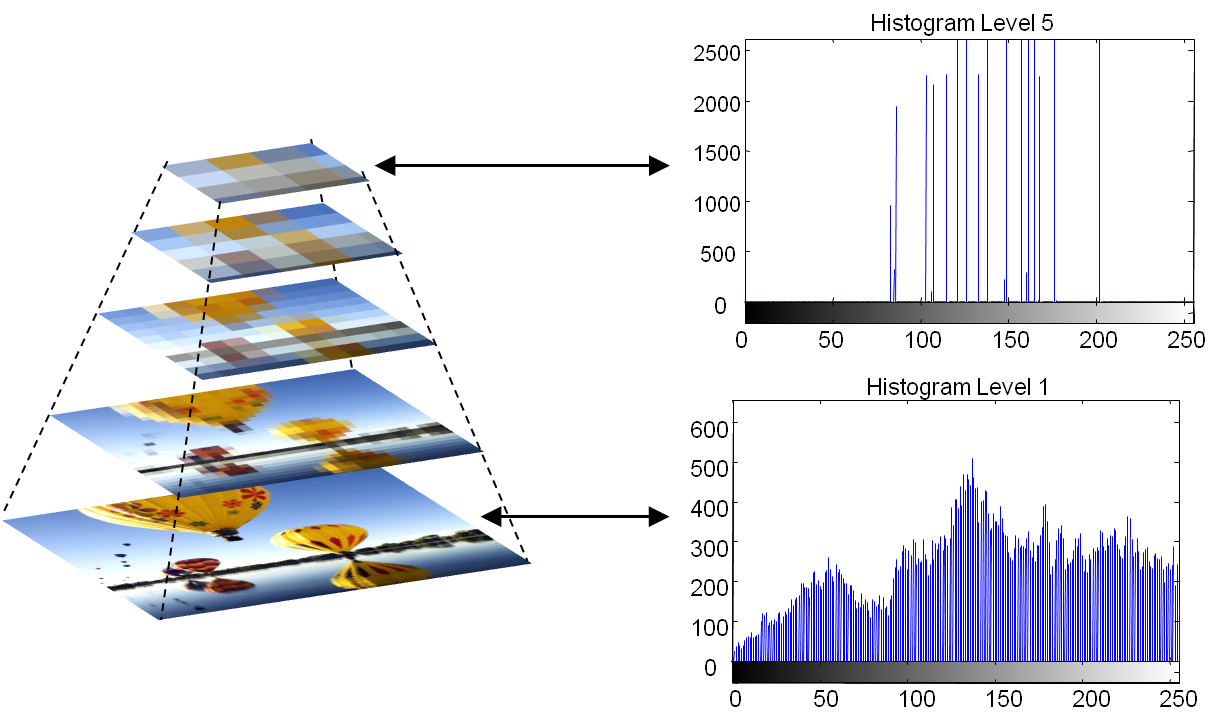
\includegraphics[width=1\textwidth]{graphic/LucasKanadePyr.png}
\caption{Lucas-Kanade-Algorithm with Pyramidal Scaling}
	\label{fig:LucasKanadePyr.png}
\end{figure}

Correlation based approaches use the strategy of searching and matching segments trough a image sequence. Such algorithms work satisfactory, if the distribution of intensity in the processed regions of the image is constant over time. Another more conventional name for this kind of algorithm is block matching (See figure \ref{fig:BlockMatching.png}). Thereby the algorithm tries to match blocks from previous to the actual image in the defined section.  The block size and the corresponding search section influences the calculation time of processing. The result of the block matching algorithm is the vector shift of the blocks. This shift can be transformed in relation to the sample rate to the velocity vector field \gls{OF}. 
\newpage
One of the biggest advantages of correlation based approaches is the simplicity of processing and the and the uncomplex mathematical theory which allows a fast and easy evaluation of the process.
Drawbacks of this approach are the memory intensity as well as the error sensibility which bases on wrong matches. Further the execution time characteristic of such approaches is related to the search algorithms and the realisation. 
Generally, all approaches introduced in this chapter can be configured and executed unprofitable to the characteristics of the incoming image sequence, which can further be a reason for unsatisfactory results.      


\begin{figure}[!h]
	\centering
		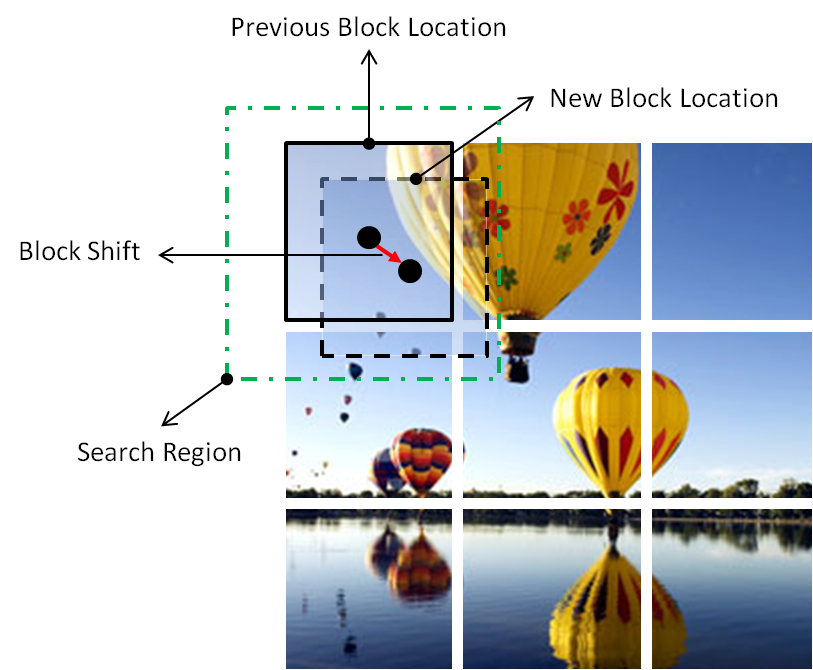
\includegraphics[width=1\textwidth]{graphic/BlockMatching.png}
\caption{Block Matching Algorithm}
	\label{fig:BlockMatching.png}
\end{figure}



% 2 Seiten Optical Flow, Definition, Algorithms,
%   Strengths and
%   problems (aperture, relative movements, photogrammetry, outliner),
%   filter(RANSAC)


\section{Control System Characteristics}
\label{mt:c:literature:s:Control_Systems_Characteristics}

This chapter focus several aspects of control systems, which are frequently used in \gls{UAV} projects. At first, different control architectures are examined, compared and discussed.
Further, several methods of analysis and design of control systems are presented with the aim to show how such systems can be 
designed, robust and stable, using different strategies in different domains. Another focus, which is introduced with the multiple domain analysis of this chapter, is the methodology and analysis of discrete time-variant control systems.

\subsection{Control Approaches} % 2 Seiten (act sum 15)(Try to Extend this chapter)

The closed loop feedback architecture is an approved method for controlling
systems, that is nearly used in the most of the systems controls in industry and
society. So the most of the researches in the \gls{UAV}~ stabilisation topic were, and
still are, executed with closed loop control architectures, which are built up as
\gls{MIMO}~ or as multiple \gls{SISO}~ systems. The differences between the researched
approaches are the amount of inputs and outputs of the physical process, the
type of controller, the used measurements and the sampling rate. Thereby the type
and behaviour of the controller is close related to the measurements and the
physical process \citeref[p.3]{DorBis01}. The classical control approach using
\gls{PID}~ controller was researched in several \gls{HUAV}~ projects
\citebib[pp.24-31]{Sik08} \citebib[pp.43-68] {Bou07}. These researches show that
the classical \gls{PID}~ controller is not robust enough to handle with complex
models which include several integration states, but has to be transformed to cascaded
\gls{PID}~ controller.
\newpage
Basically the implementation of a \gls{PID}~ controller can be executed with the
determination of three parameters for the given process. These parameters are the proportional, integral and derivative gain of the controller, which have an impact on the dynamic behaviour of the controlled value \citebib[pp. 695-698 PID Controllers]{DorBis01}.
Another approach for control improvement was introduced by
Luenberger \citebib{Lue71} and describes a closed loop control approach called state-observer, which simulates the process in real time parallel to the true
process by using the input and output vector of the closed loop system and
corrects the control strategy. Bloesch et al. \citeref[p.5] {BloWeiScaSie10} have
shown in their research, that the problem of sensors with non-negligible time
delay can be solved to an adequate result by using a state-observer. The reason
for that is that the state-observer allows to configure and to control the
stability behaviour of the closed loop feedback architecture. If a process can be
observed or furthermore controlled, is related to the possible states of the system,
and furthermore to the measurements of the \gls{DOF}~ \citeref [pp.632-636
Controllability and Observability]{DorBis01}. In the other hand a
state-observer architecture has a big impact to the calculation capacity of the \gls{UAV}~ target
because the real-time process simulation of a 6 \gls{DOF}~ rigid-body becomes very
complex.


\begin{figure}[H]
	\centering
		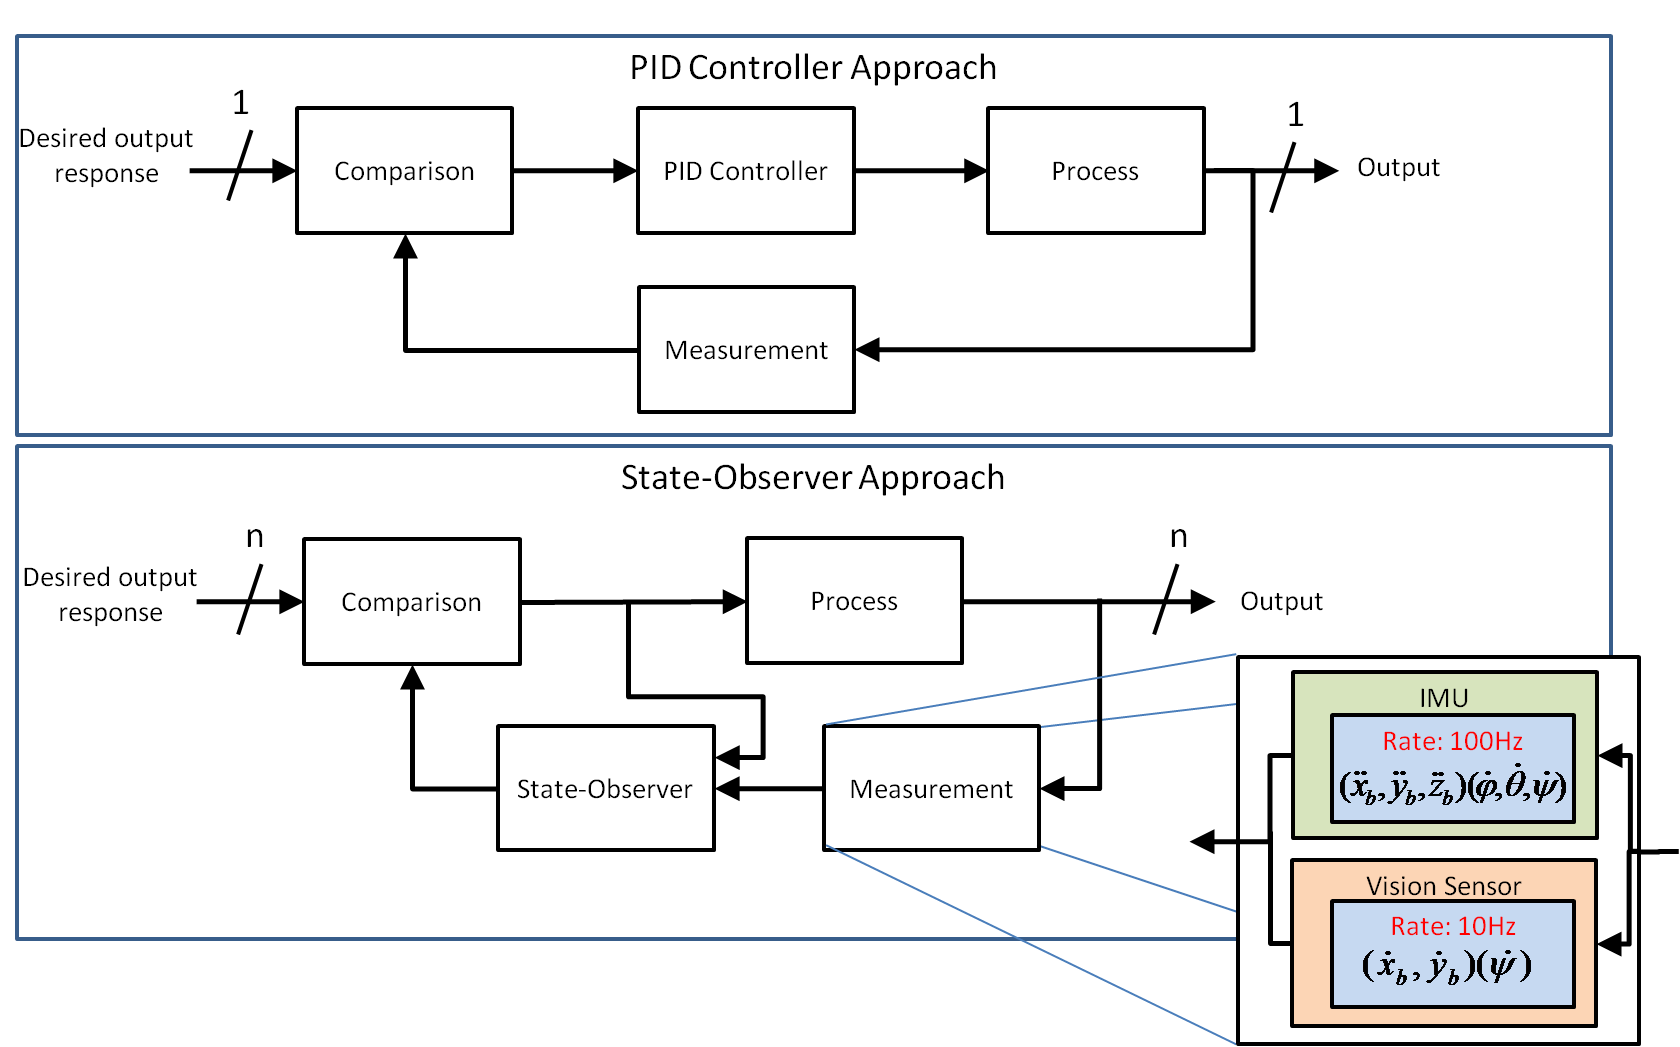
\includegraphics[width=1\textwidth]{graphic/ClosedLoopControlSyst.png}
\caption{PID-Controler and State-Observer in closed loop system with variable sample sensor rates}
	\label{fig:ClosedLoopControlSyst.png}
\end{figure}


\subsection{Performance Measures in the Time Domain}
Control systems usual are designed and evaluated in different domains under
consideration of the special behaviour of these. The closed loop feedback
architecture can be described with a transfer function, which shows the behaviour
of the closed loop feedback system in respect to the system boundaries. The time
domain is used to visualize the time variant behaviour of the controlled value
and allows definitions of performance measures. These measures are visualised in
figure \ref{fig:ControlSystemCharacteristics.png}\footnote{This picture extends
the diagram presented in \citeref[Chapter 2, p.11 Characteristics of control
systems]{KelKulLinZim07}} and can be described with the following characteristics
\footnote{The content of the characteristics is derived from \citeref[Chapter 2,
p.12 Requirements of control systems]{KelKulLinZim07}\citeref[Chapter
5, pp.228-230 The Performance of Feedback Control Systems]{DorBis01}}.


\begin{itemize}

\item Stability: A control system is called stable, if the controlled value y(t)
reaches a constant value and does not oscillate between a set of values.


\item Precision: The precision describes the ability of steady state error
minimization of a control system. The best case of precision is
\ensuremath{e(\infty)=y_{set}(\infty)-y(\infty)=0}.

\item Transient oscillation: The oscillation process of a system is described
with the needed time of the function is needed to reach the range of tolerance
\ensuremath{T_s} and is called settling time. This time depends on the rise time
which describes the first entrance point of the range of tolerance. A short rise time
can bring the disadvantage of a big maximal overshoot \ensuremath{y_{max}},
which should be kept minimal.

\item Robustness: A control system is characterized as robust, if it does not
become instable if system values change over time in scope of their tolerances.
Such tolerances can occur from temperature variations or tribological reasons.

\item Load of actuator: The load of the actuator(s) should be minimal. That means
that the maximum actuator value should be equal to the needed value to prevent
unnecessary work.
\end{itemize}

\begin{figure}[H]
	\centering
		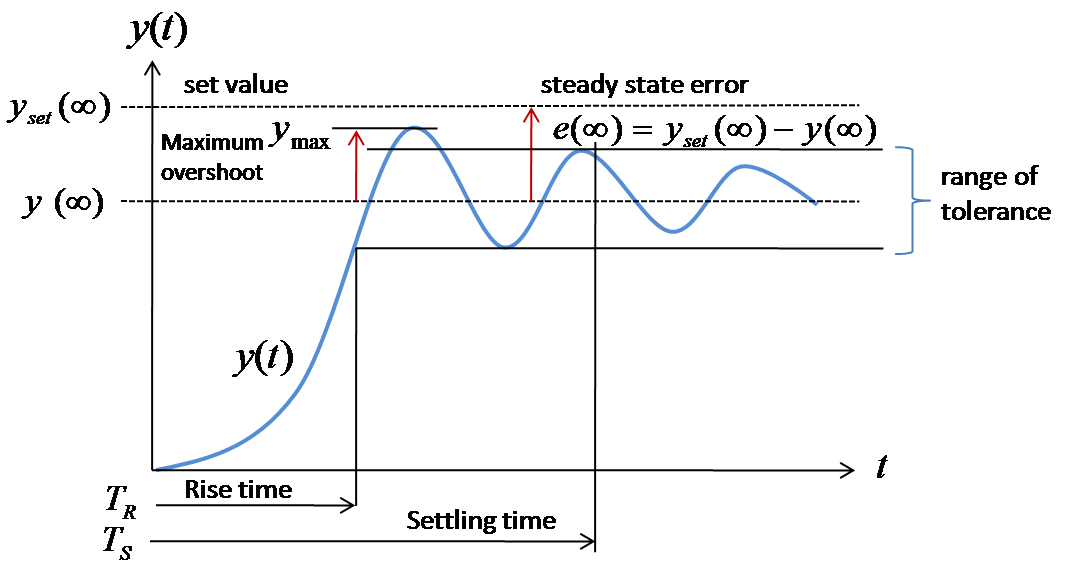
\includegraphics[width=1\textwidth]{graphic/ControlSystemCharacteristics.png}
\caption{Performance measurement values of control systems}
	\label{fig:ControlSystemCharacteristics.png}
\end{figure}


\subsection{Continuous and Discrete Time and Frequency Domains}
The necessity of the linear approximation and the simplification of
systems, led the analysts to the use of the Laplace transformation. This method
transfers relative easily solved algebraic equations in the Laplace domain for
the more differential equations in the time domain\citebib[pp.41-47 The Laplace
Transform]{DorBis01}. Combined with the fact that the sampling rate of a
computing system can have a big impact to the stability of it, the
z-transformation allows transferring functions from the continuous frequency
domain to the discrete frequency domain \citebib[pp.749-754 The
z-Transform]{DorBis01}. These two transformations and the corresponding
retransformations are visualized in the figure
\ref{fig:TimeLaplaceAndZDomain.png}\footnote{This figure bases on the theorems in
\citebib[Chapter 4, p.17 Definitions and Rules of the
z-Transform]{KelKulLinZim07}} and can be executed in a simple form by using
transformation tables
 \footnote{See Transformation tables in \citebib[pp.42 Important Laplace
 Transform Pairs]{DorBis01} and \citebib[pp.751 
z-Transforms]{DorBis01}}.
\newpage
The frequency domain equations are describes as
functions of the complex numbers. This continuous frequency parameter is discredited by using the
following abbreviation \ensuremath{z=e^{sT}} where T is the sampling rate of the
discrete system. The factor k in the discrete domain symbolizes the
\ensuremath{k^{th}} sample value of the function and can be described as
parameterization factor of the sample time T \citeref[Chapter 4, p.19 z-Domain set value transfer function of a
closed loop control system]{KelKulLinZim07}.


\begin{figure}[H]
	\centering
		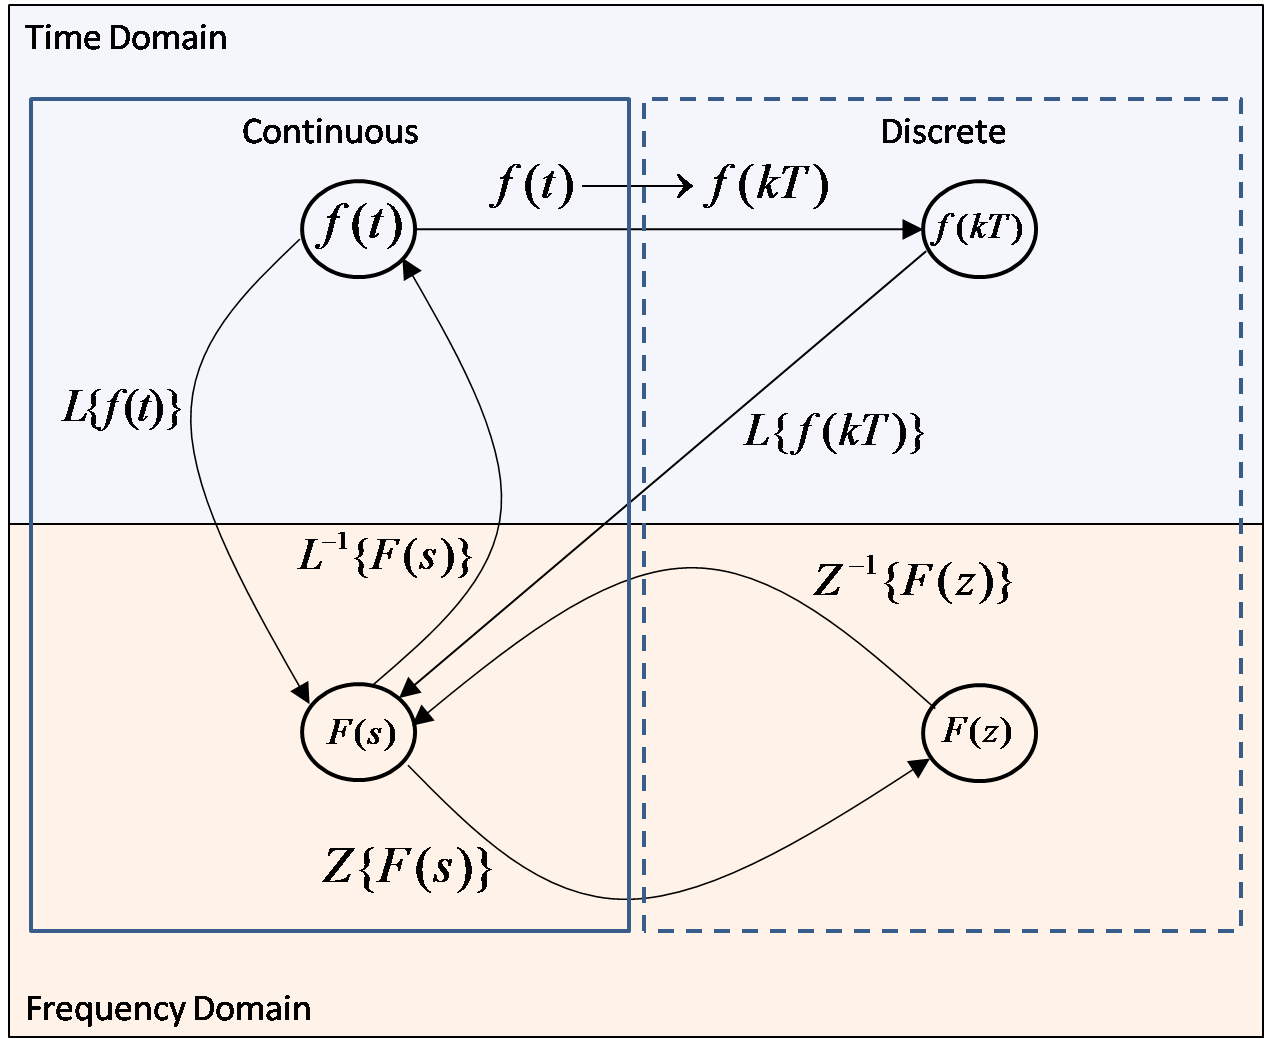
\includegraphics[width=1\textwidth]{graphic/TimeLaplaceAndZDomain.png}
\caption{Transformation possibilities of continuous and discrete time and frequency domains}
	\label{fig:TimeLaplaceAndZDomain.png}
\end{figure}
\newpage
\subsection{Stability criteria of Transfer Functions}
\label{mt:c:literature:s:Stability_criteria_of_transfer_functions}
The mentioned simplification of \gls{CLCS}~ in the following chapter can be shown by
reducing the complete system to a quotient which in contains polynomials for the
numerator and denominator.
This characteristically quotient is called \gls{TF}~ and
describes the behaviour of a system in relation to its boundaries. In the
continuous domain the \gls{TF}~ can be created as \gls{SVTF}~ (See formula
\ref{formula:TF_GW_s}) or as \gls{EVTF}~ (See \ref{formula:TF_GV_s}) which
allows investigations from two different input perspectives of the \gls{CLCS}. The
discrete closed loop control system can be used to describe the dynamic control
behaviour of a discrete controller which controls a continuous process from the
\gls{SVTF}~ perspective (See formula \ref{formula:TF_GV_z}). The interface between
the process and the controller, is realised in this example with sample and hold
components, which discretise the continuous process \citebib[p.747
Sampled-Data Systems]{DorBis01}. The figure
\ref{fig:TransferFunctions.png}\footnote{This picture extends diagrams presented in \citeref[Chapter 4, p.2 Generic linear Closed Loop Control
System]{KelKulLinZim07},\citeref[Chapter 4, p.19 z-Domain set value transfer
function of a closed loop control system]{KelKulLinZim07}, \citeref[Chapter 4,
p.21 Stability]{KelKulLinZim07}} visualizes the generic architecture of \gls{CLCS}~
in the continuous and discrete domain. Thereby the figure shows that the components
of a global \gls{TF}~ of a \gls{CLCS}~ also can be denoted as \gls{TF}~ which describe the
specific behaviour of the controller, the process \footnote{In specific literature of
control systems, sometimes the synonym plant is used for process} and
measurement\footnote{The measurement component in the discrete domain is
substituted with a sample component which holds the value of the process in the
desired appearance}.


\begin{figure}[H]
	\centering
		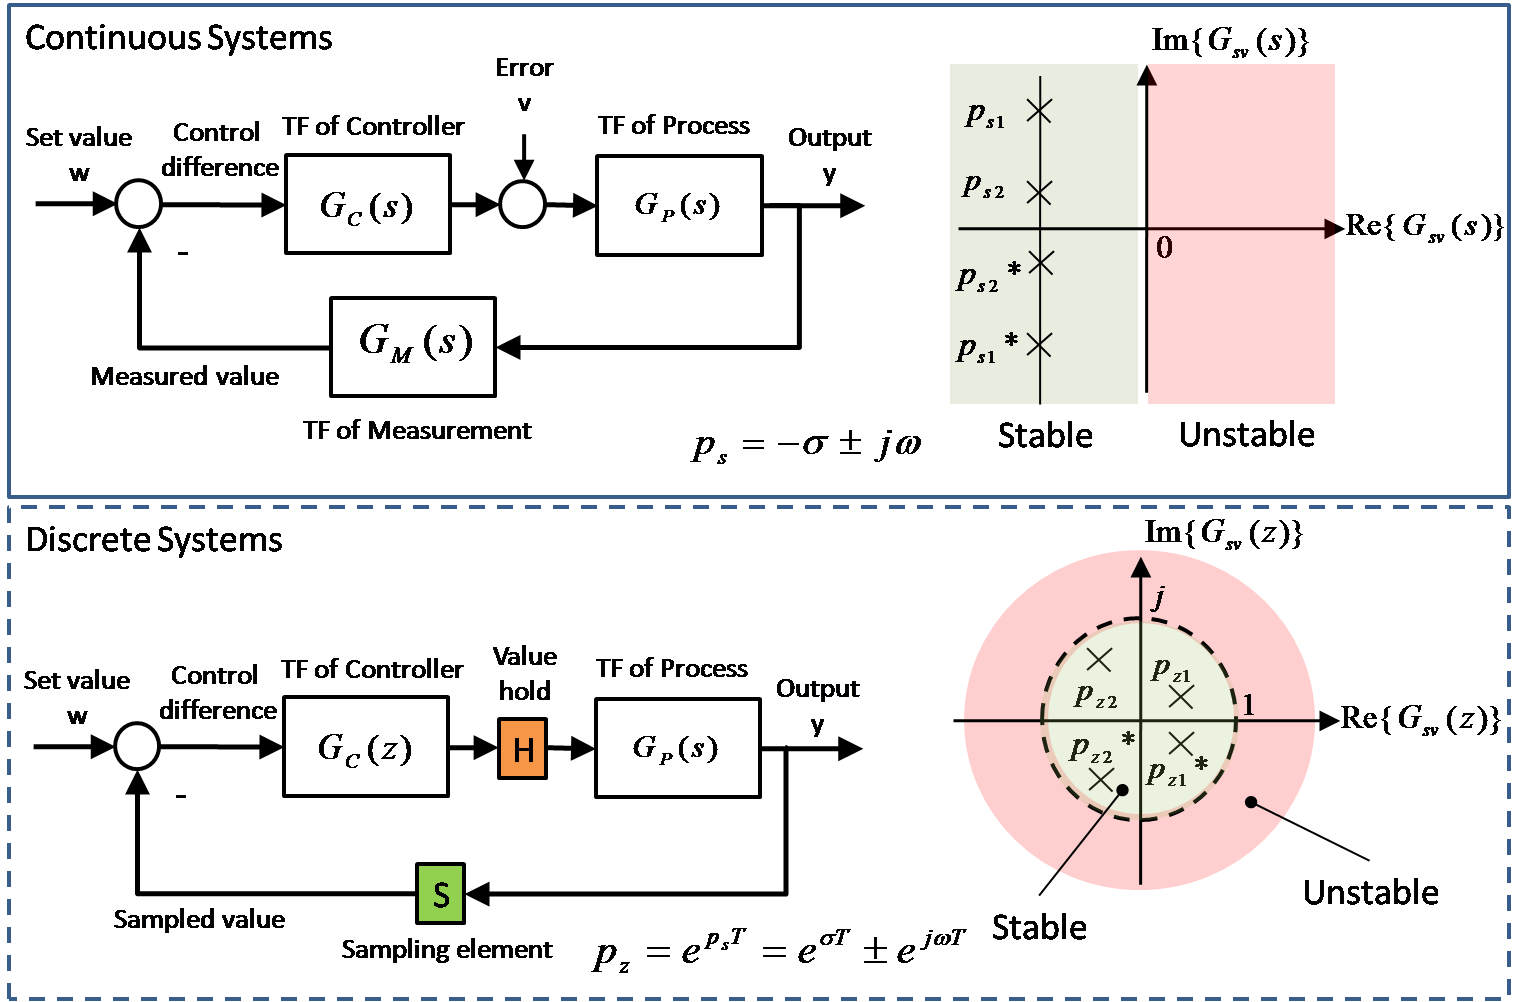
\includegraphics[width=1\textwidth]{graphic/TransferFunctions.png}
\caption{TF of continuous and discrete CLCS and their stability behaviour}
	\label{fig:TransferFunctions.png}
\end{figure}

The corresponding \gls{TF}~ of the introduced domains are shown in the formulas
\ref{formula:TF_GW_s}, \ref{formula:TF_GV_s},
\ref{formula:TF_GV_z}\footnote{See \citeref[p.754
Closed-Loop Feedback Sampled-Data Systems]{DorBis01}}. Especially the \gls{SVTF}~
contains important information of the stability behaviour. Continuous \gls{SVTF}~
are stable, if the poles \ensuremath{p_{s}} of the quotient are located at the real negative section of the complex plane. 
Equivalent to that the stability of a discrete \gls{SVTF}~ is given, if the poles \ensuremath{p_{z}} are
located in the unit circle of the complex plane \footnote{This causes the
quantisation relation of the frequency \ensuremath{z=e^{sT}}}~\footnote{\gls{CLCS}
which have poles located on the edges of the stability sections are called
semi-stable. Such \gls{CLCS} are totally not robust and also assigned to the set of
unstable systems}. 
\newpage
This stability behaviour in the complex plane is visualised in
 the figure \ref{fig:TransferFunctions.png}. Consequently the sample rate of
digital systems and the corresponding sensors has a big impact to the stability
of \gls{CLCS}~\footnote{See \citeref[p.756 Stability Analysis in the z-Plane]{DorBis01}}.

\begin{equation}
\label{formula:TF_GW_s}
G_{W}(s)=\frac{Y(s)}{W(s)}=\frac{G_{C}(s)*G_{P}(s)}{1+G_{C}(s)*G_{P}(s)*G_{M}(s)}
\end{equation}

\begin{equation}
\label{formula:TF_GV_s}
G_{V}(s)=\frac{Y(s)}{V(s)}=\frac{G_{S}(s)}{1+G_{C}(s)*G_{P}(s)*G_{M}(s)}
\end{equation}

\begin{equation}
\label{formula:TF_GV_z}
G_{W}(z)=\frac{Y(z)}{W(z)}=\frac{G_{C}(z)*G_{P}(z)}{1+G_{C}(z)*G_{P}(z)}
\end{equation}

